%% SW design: klassebeskrivelse devkit domain klasser
\newpage

\begin{figure}[htbp] \centering
{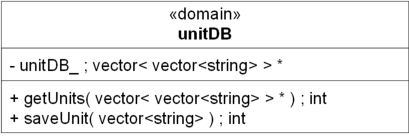
\includegraphics[scale=1.5]{filer/design/Klassediagrammer/sw_unitDB}}
\caption{Klasse unitDB}
\label{fig:unitDB klassediagram}
\end{figure} 

{\centering
\textbf{unitDB}\par
}
\textbf{Ansvar:} Gemmer opsatte Enheder og deres parametre. \

\textbf{Attributter:}
\begin{itemize}
	\item \verb+vector< vector<string> > * unitDB_+ Dynamisk allokeret \verb+vector+ til enhedsliste.
	\item \verb+int max_+ \textbf{??????}
	\item \verb+int size_+ \textbf{??????}
\end{itemize}

\verb+unitDB( ) +\\
\textbf{Parametre:} Ingen.\\
\textbf{Returværdi:} Ingen. \\
\textbf{Beskrivelse:} Allokerer dynamisk en \verb+vector< vector<string> >+ til attributten \verb+unitDB_+. Indsætter 18 enheder af typen \verb+vector<string>+ med grænserne -1 for temperatur og fugtighed, og status sættes til [Deaktiv] på hhv. index 1, 2, 3. Index 0 er nummeret på enheden. \\

\verb+~unitDB( ) +\\
\textbf{Parametre:} Ingen.\\
\textbf{Returværdi:} Ingen. \\
\textbf{Beskrivelse:} Deallokerer \verb+unitDB_+. \\

\verb+int getUnits( vector< vector<string> > * ) +\\
\textbf{Parametre:} Modtager pointer til hvor enhedslisten skal gemmes.\\
\textbf{Returværdi:} 0 ved succes ellers negativ i overenstemmelse med fejl-listen. \\
\textbf{Beskrivelse:} Skriver indholdet af \verb+unitDB_+ over i den modtagne pointer. \\

\verb+int saveUnit( vector<string> ) +\\
\textbf{Parametre:} \verb+vector+ som skal gemmes \\
\textbf{Returværdi:} 0 ved succes ellers negativ i overenstemmelse med fejl-listen. \\
\textbf{Beskrivelse:} Finder enhedsnummer fra modtagne vektor og gemmer data i den pågældende plads i \verb+unitDB_+. \\

\begin{figure}[htbp] \centering
{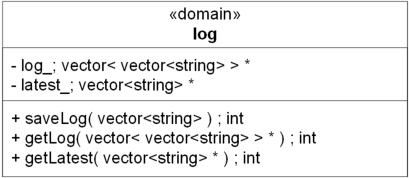
\includegraphics[scale=1.5]{filer/design/Klassediagrammer/sw_log}}
\caption{Klasse log}
\label{fig:log klassediagram}
\end{figure} 

{\centering
\textbf{log}\par
}
\textbf{Ansvar:} Gemmer log-information fra tilkoblede Enheder. \

\textbf{Attributter:}
\begin{itemize}
	\item \verb+vector< vector<string> > * log_+ Dynamisk allokeret \verb+vector+ til loggen.
	\item \verb+vector<string> * latest_+ Dynamisk allokeret \verb+vector+ til senest loggede information.
\end{itemize}

\verb+log( ) +\\
\textbf{Parametre:} Ingen \\
\textbf{Returværdi:} Ingen\\
\textbf{Beskrivelse:} Allokerer dynamisk en \verb+vector< vector<string> >+ til \verb+log_+ og en \verb+vector<string>+ til \verb+latest_+. \\

\verb+~log( ) +\\
\textbf{Parametre:} Ingen \\
\textbf{Returværdi:} Ingen\\
\textbf{Beskrivelse:} Deallokerer \verb+log_+ og \verb+latest_+. \\

\verb+int saveLog( vector<string> ) +\\
\textbf{Parametre:} \verb+vector+ som skal gemmes. \\
\textbf{Returværdi:} 0 ved succes ellers negativ i overenstemmelse med fejl-listen. \\
\textbf{Beskrivelse:} Gemmer modtaget data ved at pushe \verb+log_+ og overskrive \verb+latest+. \\

\verb+int getLog( vector< vector<string> > * ) + \\
\textbf{Parametre:} Pointer til hvor data skal gemmes. \\
\textbf{Returværdi:} 0 ved succes ellers negativ i overenstemmelse med fejl-listen. \\
\textbf{Beskrivelse:} Skriver data fra \verb+log_+ over i modtagne pointer. \\

\verb+int getLatest( vector<string> * ) +\\
\textbf{Parametre:} Pointer til hvor data skal gemmes.  \\
\textbf{Returværdi:} 0 ved succes ellers negativ i overenstemmelse med fejl-listen. \\
\textbf{Beskrivelse:} Skriver data fra \verb+latest_+ over i modtagne pointer. \\


